\subsection{Равносоставленность}
\begin{definition}
    Два многоугольника $W_1, W_2$ \textit{равносоставлены}, если существуют многоугольники $M_1, \dots, M_n$ такие, что:
    \begin{enumerate}
        \item $\forall i, j \ M_i \cap M_j = \emptyset$;
        \item $\bigcup_{i=1}^n M_i = W_1, \ \bigcup_{j=1}^n M_j = W_2$.
    \end{enumerate} 
\end{definition}

\begin{theorem}[Бойяи-Гервин]
    Два многоугольника на плоскости равносоставлены тогда и только тогда, когда они равновеликие.
\end{theorem}
\begin{proof}
    %Доказательство будет на семинарах (надеюсь, я ничего не перепутал, и это именно данная теорема ушла на семинары).
    $\underline{\Longrightarrow}$ Если два многоугольника $P$ и $Q$ равносоставлены, то существует разбиение каждого из них на конечное количество многоугольников $P_1, \dots, P_n$ и $Q_1, \dots, Q_n$, причём $\forall i \ P_i$ конгруэнтен $Q_i$. Поскольку конгруэнтные фигуры имеют равную площадь, то получаем, что и площади $P$ и $Q$ равны.

    $\underline{\Longleftarrow}$ Пусть $P$ и $Q$ — два многоугольника с равными площадями. Покажем, что их можно разбить на конгруэнтные части. Воспользуемся тем фактом, что любой многоугольник можно разбить на треугольники (сам факт проверяется индукцией по числу вершин). Также воспользуемся тем, что отношение равносоставленности является отношением эквивалентности (проверяется по определению: рефлексивность, симметричность, транзитивность).

    Разрежем теперь многоугольник на треугольники. Любой треугольник равносоставлен с параллелограммом (см.рис.\ref{fig:c8.1}) (делим треугольник по средней линии).

    \begin{figure}[htbp]
        \centering
        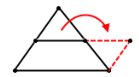
\includegraphics[scale=1]{images/c8.1.png}
        \caption{Равносоставленность треугольника и параллелограмма.}
        \label{fig:c8.1}
    \end{figure}

    Любой параллелограмм равносоставлен с прямоугольником (см.рис.\ref{fig:c8.2}), поэтому любые два параллелограмма равной площади и с равным основанием равносоставлены.

    \begin{figure}[htbp]
        \centering
        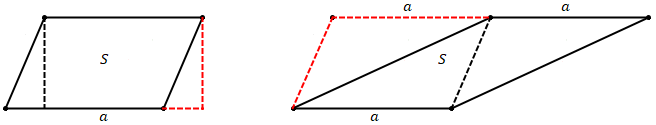
\includegraphics[scale=0.7]{images/c8.2.png}
        \caption{Равносоставленность параллелограмма и прямоугольника.}
        \label{fig:c8.2}
    \end{figure}

    \begin{figure}[H]
        \centering
        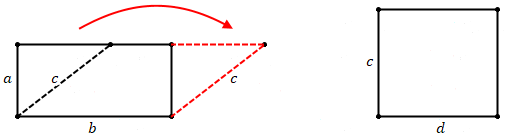
\includegraphics[scale=0.7]{images/c8.3.png}
        \caption{Равносоставленность прямоугольников равной площади.}
        \label{fig:c8.3}
    \end{figure}

    Два любые прямоугольника равной площади равносоставлены (см.рис.\ref{fig:c8.3}) — доказывается сведением к предыдущему шагу. Следовательно, прямоугольник площади $S$ равносоставлен прямоугольнику со сторонами 1 и $S$. Тогда и произвольный многоугольник площади $S$ равносоставлен прямоугольнику со сторонами 1 и $S$. Пользуясь свойством транзитивности, получаем, что равновеликие многоугольники равносоставлены.
\end{proof}


\begin{theorem}[Ден]
    Куб и правильный тетраэдр равного объёма не равносоставлены.
\end{theorem}

\begin{definition}
    Функция $f$, определённая на множестве $M \subset \R$, называется \textit{аддитивной}, если $\forall n_1 x_1 + \dots + n_k x_k = 0, \ n_i \in \Z, \ x_i \in M$ выполнено $$n_1 f(x_1) + \dots + n_k f(x_k) = 0.$$ 
\end{definition}

\begin{definition}
    Пусть дан $W$ — многогранник. $\alpha_1, \dots, \alpha_k$ — величины его двугранных углов, $a_1, \dots, a_k$ — длины его рёбер. Пусть дана аддитивная функция $f$, определённая на множестве $M: \{\alpha_1, \dots, \alpha_k, \pi\} \in M$, причём $f(\pi) = 0$. Тогда \textit{инвариантом Дена} многогранника $W$ назовём число $f(W) = \sum a_i f(\alpha_i)$ — сумма по всем рёбрам.
\end{definition}

\begin{statement}
    Любой инвариант Дена для куба равен нулю.
\end{statement}
\begin{proof}
    % $$2 \cdot \frac{\pi}{2} - \pi = 0$$
    % $$2 \cdot f \left(\frac{\pi}2\right) - 1 \cdot f(\pi) = 0 \Rightarrow f \left(\frac{\pi}2\right) = 0 \Rightarrow f(\text{куб}) = 6 \cdot 0 = 0.$$
    \[f(\text{куб}) = \sum_{i = 1}^{12} a \cdot f\left(\frac{\pi}2\right) = 12 a \cdot f\left(\frac{\pi}2\right).\]
    Воспользуемся аддитивностью: 
    \[4 \cdot \frac{\pi}2 = 2 \pi \Longrightarrow 4 f\left(\frac{\pi}2\right) = f(2 \pi) = f(\pi + \pi) = f(\pi) + f(\pi) = 0 + 0 = 0\]
    Поэтому \[f(\text{куб}) = 12 a \cdot 0 = 0.\]
    Следовательно, любой инвариант Дена для куба равен нулю.
\end{proof}

\begin{statement}
    Инвариант Дена для призмы равен нулю.
\end{statement}
\begin{proof}
    \begin{figure}[htbp]
        \centering
        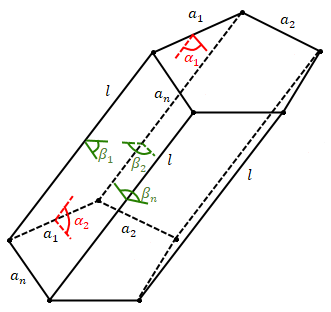
\includegraphics[scale=1]{images/c8.9.png}
        \caption{Призма.}
        \label{fig:c8.9}
    \end{figure}
    Ребро может быть либо боковым (длины $l$), либо ребром основания (длины $a_i$). Рассмотрим рёбра основания длины $a_1$ и двугранные углы при этих рёбрах $\alpha_1, \alpha_2$. Так как основания призмы параллельны, то $\alpha_1 + \alpha_2 = \pi$. Тогда
    \[a_1 f(\alpha_1) + a_1 f (\alpha_2) = a_1 f(\alpha_1 + \alpha_2) = a_1 f(\pi) = 0.\]
    Рассмотрим боковые рёбра: пусть $\beta_1, \dots, \beta_n$ — двугранные углы при боковых рёбрах. Тогда
    \[l f(\beta_1) + \dots + l f(\beta_n) = l f(\beta_1 + \dots + \beta_n).\]
    Сумма углов $n$-угольника равна $\pi(n-2)$, поэтому 
    \[l f(\beta_1 + \dots + \beta_n) = l f(\pi(n-2)) = l(n-2)f(\pi) = 0.\]
    Следовательно, для любой аддитивной функции инвариант Дена равен нулю. 
\end{proof} 

\begin{theorem}[Хадвигер]
    Пусть $W_1, W_2$ — два многогранника, $f$ — аддитивная функция, область определения которой включает число $\pi$ и величины всех двугранных углов $W_1, W_2$. Пусть $f(W_1) \neq f(W_2)$. Тогда $W_1, W_2$ не равносоставлены.
\end{theorem}

\begin{remark}
    Через эту теорему будем доказывать теорему Дена.
\end{remark}

% \begin{proof}
%     Тише едешь — дальше будешь. Что-то с тетраэдром и утверждением о том, что $cos(m \alpha) = \frac{a_m}{3^m}, \ a_m \text{не делится на} 3, \ a_m \in Z$
% \end{proof}

\begin{proof}[Доказательство теоремы Дена]
    Зададим некоторую аддитивную функцию, содержащую величины всех двугранных углов куба $\left(\frac{\pi}{2}\right)$ и правильного тетраэдра $\left(\phi = \arccos{\frac{1}{3}}\right)$, т.е. зададим функцию на множестве $M = \left\{\frac{\pi}{2}, \pi, \arccos{\frac{1}{3}}\right\}$.
    Так как по условию $f(\pi) = 0$, то и $f(\frac{\pi}{2}) = 0$. Примем $f(\phi) = 1$. Посчитаем значение инварианта Дена для этой аддитивной функции для куба и правильного тетраэдра:
    \[f(\text{куб}) = 12 f\left(\frac{\pi}{2}\right) = 0,\]
    \[f(\text{тетраэдр}) = 6bf(\phi) = 6b \neq 0.\]

    Осталось проверить, что функция, которую мы задали, действительно будет аддитивной. Для любой зависимости вида $$n_1 \pi + n_2 \phi = 0$$ должно выполняться соотношение $$n_1 f(\pi) + n_2 f(\phi) = 0.$$

    Так как $f(\pi) = 0$, а $f(\phi) \neq 0$, это соотношение может быть выполнено только при $n_2 = 0$, иными словами, функция будет аддитивной, если не существует зависимостей вида $n_1 \pi + n_2 \phi = 0$ при $n_2 \neq 0$. Это равносильно следующему утверждению (на лекции был другой пример (вроде), но не суть):

    \begin{lemma}
        Число $\frac{\phi}{\pi}$ иррационально.
    \end{lemma} 
    \begin{proof}
        Пусть $$\frac{\phi}{\pi} = \frac{1}{\pi} \arccos{\frac{1}{3}} = \frac{p}{q} \in \Q$$ — несократимая дробь.
        Пусть также $$\cos{\phi} = \frac{m}{n} \in \Q$$ — несократимая дробь (в нашем случае $\cos{\phi} = \frac{1}{3}$).
        Воспользуемся формулой косинуса двойного угла: если $\cos{\alpha} = \frac{k}{l} \in \Q$, то
        $$\cos{2\alpha} = 2 \frac{k^2}{l^2} - 1 = \frac{2k^2 - l^2}{l^2}$$ — НОД числителя и знаменателя равен 1 либо 2. Но при $l > 2$ выполнено $\frac{l^2}{2} > l$. Поэтому в последовательности $$\cos{\phi}, \cos{2\phi}, \cos{4\phi}, \cdots, \cos{2^r \phi}, \cdots$$ нет повторяющихся чисел (так как знаменатели дробей возрастают).

        С другой стороны, в последовательности
        $$\phi, 2\phi, 4\phi, \cdots, 2^r \phi, \cdots$$
        будут углы, равные по модулю $2 \pi$: действительно, если $\phi = \frac{p}{q} \pi$, то в последовательности
        $$\frac{p}{q} \pi, 2 \frac{p}{q} \pi, 4 \frac{p}{q} \pi, \cdots, 2^r \frac{p}{q} \pi, \cdots$$
        может быть всего $2q - 1$ различных числа (по модулю $2 \pi$), поэтому достаточно взять $r = 2q$.

        Получили противоречие — у чисел, равных по модулю $2 \pi$, косинусы должны быть равны, но в последовательности, содержащей косинусы этих чисел, нет одинаковых членов.
    \end{proof}
    Тем самым, лемма доказана, а значит, доказана и аддитивность $f$. Поэтому (по теореме Хадвигера) куб и правильный тетраэдр не равносоставлены, и теорема Дена доказана.
\end{proof}

\begin{proof}[Доказательство теоремы Хадвигера]

\begin{lemma}[1]
    Пусть $f$ — аддитивная функция, определённая на множестве $M: \ \alpha \in \R, \ \alpha \notin M$. Тогда существует аддитивная функция $\tilde{f_i}$, определённая на $M \cup \{\alpha\}$ такая, что $\forall x \in M: \ f(x) = \tilde{f}(x)$
\end{lemma}
\begin{proof}
    Будем считать, что $M = \{\alpha_1, \dots, \alpha_k\}$.
    \begin{enumerate}
        \item Если нет зависимости вида 
        \[n_1 \alpha_1 + \dots + n_k \alpha_k + m \gamma = 0,\]
        где $m \neq 0$, то положим $\tilde{f}(\gamma)$ равным любому числу.
        \item Пусть есть зависимость вида 
        \[n_1 \alpha_1 + \dots + n_k \alpha_k + m \gamma = 0,\]
        где $m \neq 0$. Тогда положим
        \[\tilde{f}(\gamma) = - \left(\frac{n_1}{m}\right) f(\alpha_1) - \dots - \left(\frac{n_k}{m}\right) f(\alpha_k).\]
    \end{enumerate}

    Проверим, что тогда для любой зависимости вида
    \[p_1 \alpha_1 + \dots + p_k \alpha_k + l \gamma = 0\]
    будет выполнено соотношение
    \[p_1 \tilde{f}(\alpha_1) + \dots + p_k \tilde{f}(\alpha_k) + l \tilde{f}(\gamma) = 0.\]
    Получим
    \begin{multline*}
        (n_1 \alpha_1 + \dots + n_k \alpha_k + m \gamma) l - (p_1 \alpha_1 + \dots + p_k \alpha_k + l \gamma) m = \\= (n_1 l - p_1 m) \alpha_1 + \dots + (n_k l - p_k m) \alpha_k = 0
    \end{multline*}

    — зависимость на $M$. Так как $f$ — аддитивная функция на $M$, то получаем, что выполнено соотношение 
    \[(n_1 l - p_1 m) f(\alpha_1) + \dots + (n_k l - p_k m) f(\alpha_k) = 0,\]
    откуда
    \[l(n_1 f(\alpha_1) + \dots + n_k f(\alpha_k)) - m (p_1 f(\alpha_1) + \dots + p_k f(\alpha_k)) = 0.\]
    Так как 
    \[n_1 f(\alpha_1) + \dots + n_k f(\alpha_k) = -m \tilde{f}(\gamma),\]
    получаем
    \[-lm \tilde{f}(\gamma) - m(p_1 f(\alpha_1) + \dots + p_k f(\alpha_k)) = 0.\]
    Сокращая на $m$ и меняя знак, получаем
    \[p_1 \tilde{f}(\alpha_1) + \dots + p_k \tilde{f}(\alpha_k) + l \tilde{f}(\gamma) = 0,\]
    что и требовалось.
    
    % Если между $\alpha$ и числами из $M$ нет зависимости, то $\tilde{f}(\alpha)$ — любое число. Пусть зависимость есть, то есть существуют целые $n_0, \dots, n_k$: $$n_0 \alpha + n_1 x_1 + \dots + n_k x_k = 0 \ x_i \in M, \ n_0 \neq 0.$$
    % Тогда $f(\alpha) := - \frac{n_1 f(x_1) + n_2 f(x_2) + \dots + n_k f(x_k)}{n_0}$. Пусть есть другая зависимость $m_0 \alpha + m_1 y_1 + \dots + m_l y_l = 0, \ y_j \in M, \ m_0 \neq 0$. Верно ли $0 = m_0 f(\alpha) + m_1 f(y_1) + \dots + m_l f(y_l) = - \frac{m_0}{n_0} \left(n_1 f(x_1) + \dots + n_k f(x_k)\right) + m_1 f(y_1) + \dots + m_l f(y_l) = \frac{-m_0 n_1 f(x_1) - \dots - m_0 n_k f(x_k) + n_0 m_1 f(y_1) + \dots + n_0 m_l f(y_l)}{n_0}$?
    % $$-m_0 n_1 x_1 - \dots - m_0 n_k x_k + m_0 n_0 y_1 + \dots + m_l n_0 y_l = 0$$
    % Дополнено будет позже.
\end{proof}

\begin{lemma}[2]
    Пусть $A$ — многогранник, состоящий (разбитый в объединение непересекающихся) из многогранников $P_1, \dots, P_k$. $f$ — аддитивная функция, определённая на $\pi$ ($f(\pi) = 0$) и всех двугранных углах многогранников $A,P_1, \dots, P_k$. Тогда $f(A) = \sum f(P_i)$.
\end{lemma}
\begin{proof}
    \begin{figure}[htbp]
        \centering
        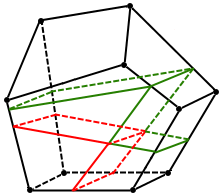
\includegraphics[scale=0.7]{images/c8.4.png}
        \caption{Многогранник $A$ состоит из многогранников $P_1, \dots, P_k$.}
        \label{fig:c8.4}
    \end{figure}

    Рассмотрим разбиение рёбер многогранников $P_1, \dots P_k$ на «звенья», заданное вершинами этих многогранников и точками пересечения рёбер.

    \begin{figure}[htbp]
        \centering
        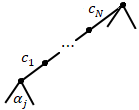
\includegraphics[scale=0.7]{images/c8.5.png}
        \caption{Разбиение ребра на звенья.}
        \label{fig:c8.5}
    \end{figure}

    Рассмотрим сумму
    \[\sum_{i,j} c_i f(\alpha_j)\]
    по всем звеньям, получившимся при разбиении многогранника $A$ на многогранники $P_1, \dots P_k$, и всем двугранным углам при этих звеньях.

    С одной стороны, эта сумма равна сумме инвариантов Дена для всех многогранников $P_1, \dots P_k$, так как 
    \[c_1 f(\alpha_j) + \dots + c_N f(\alpha_j) = l f(\alpha_j),\]
    где $l$ — длина некоторого ребра какого-то из многогранников $P_1, \dots, P_k$, а $\alpha_j$ — двугранный угол при этом ребре. Суммируя по всем звеньям, принадлежащим этому многограннику, получим значение инварианта Дена для этого многогранника. Поступая так для каждого многогранника $P_1, \dots P_k$, получим
    \[\sum_{i,j} c_i f(\alpha_j) = f(P_1) + \dots + f(P_k).\]

    С другой стороны, все звенья можно разбить на три класса:
    \begin{enumerate}
        \item звено внутри $A$;
        \item звено на грани $A$;
        \item звено на ребре $A$.
    \end{enumerate}
    
    \begin{enumerate}
        \item Подсчитаем, какой вклад в сумму будут давать звенья, лежащие внутри $A$:
        \begin{figure}[htbp]
            \centering
            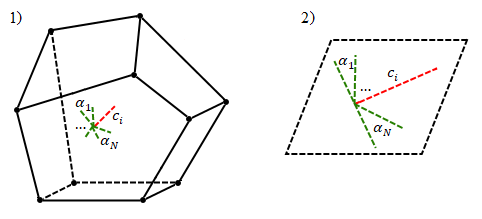
\includegraphics[scale=0.7]{images/c8.6.png}
            \caption{Звено $c_i$ лежит внутри многогранника.}
            \label{fig:c8.6}
        \end{figure}
        Возможны два случая:
        \begin{enumerate}
            \item когда звено не лежит на грани другого многогранника (см.рис.\ref{fig:c8.6}), тогда \[\sum_{j = 1}^{N} \alpha_j = 2 \pi;\]
            \item когда звено лежит на грани другого многогранника (см.рис.\ref{fig:c8.6}), тогда \[\sum_{j = 1}^{N} \alpha_j = \pi.\]
            Так как \[f(\pi) = f(2 \pi) = 0,\]
            получаем (из аддитивности функции), что
            \[c_i \sum_{j = 1}^{N} f(\alpha_j) = 0.\]
        \end{enumerate}
        \item Подсчитаем, какой вклад в сумму будут давать звенья, лежащие на грани $A$:
        \begin{figure}[htbp]
            \centering
            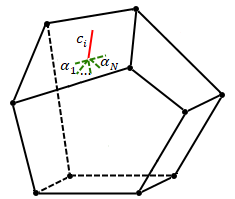
\includegraphics[scale=0.7]{images/c8.7.png}
            \caption{Звено $c_i$ лежит на грани многогранника.}
            \label{fig:c8.7}
        \end{figure}
        В этом случае \[\sum_{j = 1}^{N} \alpha_j = \pi,\]
        и (по тем же соображениям, что и в первом пункте)
        \[c_i \sum_{j = 1}^{N} f(\alpha_j) = 0.\]
        \item Подсчитаем, какой вклад в сумму будут давать звенья, лежащие на ребре $A$:
        \begin{figure}[htbp]
            \centering
            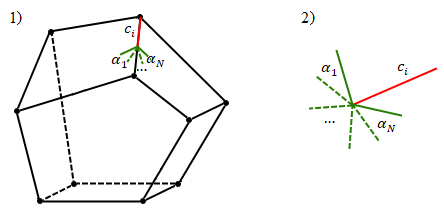
\includegraphics[scale=0.7]{images/c8.8.png}
            \caption{Звено $c_i$ лежит на ребре многогранника.}
            \label{fig:c8.8}
        \end{figure}
        В зависимости от величины двугранного угла $\beta$ при ребре, на котором лежит рассматриваемое звено, получаем два случая (в зависимости от того, больше или меньше $\beta$ развёрнутого угла):
        \begin{enumerate}
            \item $\beta < \pi$. Тогда \[\sum_{j = 1}^{N} \alpha_j = \beta.\]
            \item $\beta > \pi$. Тогда \[\sum_{j = 1}^{N} \alpha_j = \beta - \pi.\]
        \end{enumerate}
        Из условия $f(\pi) = 0$ и условия аддитивности функции, получаем
        \[c_i \sum_{j = 1}^{N} f(\alpha_j) = c_i f(\beta).\]
        Суммируя по всем звеньям этого ребра, мы получим $lf(\beta)$, где $l$ — длина ребра:
        \[\sum_i c_i f(\beta) = l f(\beta).\]
        Суммируя по всем рёбрам многогранника $A$, получим $f(A)$
        \[\sum_i l_i f(\beta_i) = f(A).\]
        Таким образом, верно равенство 
        \[f(A) = f(P_1) + \dots + f(P_k).\]
    \end{enumerate}
    
\end{proof}

\begin{remark}
    Из лемм (1)-(2) будет следовать теорема Хадвигера.
\end{remark}
\end{proof}